\documentclass{article}\usepackage[]{graphicx}\usepackage[]{color}
% maxwidth is the original width if it is less than linewidth
% otherwise use linewidth (to make sure the graphics do not exceed the margin)
\makeatletter
\def\maxwidth{ %
  \ifdim\Gin@nat@width>\linewidth
    \linewidth
  \else
    \Gin@nat@width
  \fi
}
\makeatother

\definecolor{fgcolor}{rgb}{0.345, 0.345, 0.345}
\newcommand{\hlnum}[1]{\textcolor[rgb]{0.686,0.059,0.569}{#1}}%
\newcommand{\hlstr}[1]{\textcolor[rgb]{0.192,0.494,0.8}{#1}}%
\newcommand{\hlcom}[1]{\textcolor[rgb]{0.678,0.584,0.686}{\textit{#1}}}%
\newcommand{\hlopt}[1]{\textcolor[rgb]{0,0,0}{#1}}%
\newcommand{\hlstd}[1]{\textcolor[rgb]{0.345,0.345,0.345}{#1}}%
\newcommand{\hlkwa}[1]{\textcolor[rgb]{0.161,0.373,0.58}{\textbf{#1}}}%
\newcommand{\hlkwb}[1]{\textcolor[rgb]{0.69,0.353,0.396}{#1}}%
\newcommand{\hlkwc}[1]{\textcolor[rgb]{0.333,0.667,0.333}{#1}}%
\newcommand{\hlkwd}[1]{\textcolor[rgb]{0.737,0.353,0.396}{\textbf{#1}}}%
\let\hlipl\hlkwb

\usepackage{framed}
\makeatletter
\newenvironment{kframe}{%
 \def\at@end@of@kframe{}%
 \ifinner\ifhmode%
  \def\at@end@of@kframe{\end{minipage}}%
  \begin{minipage}{\columnwidth}%
 \fi\fi%
 \def\FrameCommand##1{\hskip\@totalleftmargin \hskip-\fboxsep
 \colorbox{shadecolor}{##1}\hskip-\fboxsep
     % There is no \\@totalrightmargin, so:
     \hskip-\linewidth \hskip-\@totalleftmargin \hskip\columnwidth}%
 \MakeFramed {\advance\hsize-\width
   \@totalleftmargin\z@ \linewidth\hsize
   \@setminipage}}%
 {\par\unskip\endMakeFramed%
 \at@end@of@kframe}
\makeatother

\definecolor{shadecolor}{rgb}{.97, .97, .97}
\definecolor{messagecolor}{rgb}{0, 0, 0}
\definecolor{warningcolor}{rgb}{1, 0, 1}
\definecolor{errorcolor}{rgb}{1, 0, 0}
\newenvironment{knitrout}{}{} % an empty environment to be redefined in TeX

\usepackage{alltt}
\usepackage{hyperref}

\title{Environmental Project Work Flow using Raspberry Pi}
\author{Marc Los Huertos \& Anna Burns}
\IfFileExists{upquote.sty}{\usepackage{upquote}}{}
\begin{document}
\maketitle

\section{Using the Pi for Environmental Monitoring}

\subsection{Learning about the Raspberry Pi}

To promote relatively short documents, I have linked various pages that you can with individually: 

\begin{enumerate}

\item \href{https://github.com/marclos/UAV/blob/1aa3b3c0816f86d09fffcdab50d768257d20d80f/Hardware/Raspberry_Pi/Raspberry_Pi_Guide.pdf}{Starting work with a Raspberry Pi}

\item \ref{TBD}{TBD}

\end{enumerate}

\subsection{Sensors}

Sensors are necessary to detect the components of the air. These are used e.g. in smoke detectors. 

\subsection{The General-Purpose Input-Output}

The GPIO provides a flexible way to connect sensors to a Raspberry Pi. 

\subsection{Selecting Sensors}


\subsection{Basic Wiring}




%\subsubsection{Weather and Climate}

\subsubsection{Signal and Voltage Coverters}

All MQ-X sensors return analog signals, which we can not easily read at the Raspberry Pi. We will need an analog-to-digital converter (ADC), which can be read out via the I2C bus. In addition, we also need a logic level converter.

\begin{description}
\item[Analog-Digital Converter (8 Port)] Analog electronics vary in power (voltage or amps?) from zero to some maxium. But to read these values, we can use a small chip to convert the voltages >?< to a digital output. Without getting too complicates, this chip using a series of resisters to measure the voltage and convert it into a digital signal of 1s and 0s. A two bit A/D converter will have 0, 01, 10, 11 as output levels. Not much detail there!  So, we'll look for something with more precision...

Microchip MCP3008-I/P 10-Bit ADC with SPI  

What is SPI?

This has 8x2 pins, why?

\item[5V to 3.3V Logic Level Converter -- LLC] 
Digital input/output signals are 3.3 volts, but sensors might need 5 volts to power them.

This is not a problem if you are connecting many standard modules like the SR-04 distance sensor or the DHT11 temperature sensor, since these also use 5V to communicate with the Arduino.

But more recent modules now use 3.3V digital power, and can be damaged if connected directly to an Arduino models that uses 5V to communicate with external modules.

This is where the Logic Level Converter comes in, it takes a 5V signal and converts it to a safe 3.3V signal.

Most of these modules are bi-directional, meaning they will also convert back the 3.3V signal to 5V. \href{https://learn.sparkfun.com/tutorials/bi-directional-logic-level-converter-hookup-guide}{Bi Directional LLC}

A Logic Level Converter is easy to connect and use since it doesn’t need any programming, all you have to do is connect the 5V wire on one side and the 3.3V on the other.

Take note that some 3.3V sensors and module can be 5V tolerant, but if you want to make sure just insert a Logic Level Converter.

\item[Breadboard] Breadboards are testing platforms to build circuts. The have rows and columns which are electrically connected to give desing flexibility. There are usually two or four rails or bus strips on the long sides of the board that are for power, in our case 3.5 or 5 volts, which is usually red. The ground, usually on the inside of this power is usually blue or back colored. The rows in the inside are electrically connected, with a break in the center line. The center line is often strattled by a DIP (dual in-line package), so you can connect to each of the pins from both sides of the breadboard independently. Watch this \href{https://www.google.com/search?q=how+to+breadboards+work&rlz=1C1CHBD_enUS834US834&oq=how+to+breadboards+work&aqs=chrome..69i57j0l3.5628j1j7&sourceid=chrome&ie=UTF-8#kpvalbx=_Gz39Xq2-CuTi9APB3JGYCQ52}{Youtube video describing breadboards} for more information. 
\item[Jumper wire] is a wire the is used to connect various electronic components. For example, a jumper wire will connect our Raspberry Pi to the breadboard, various components on the breadboard, and various sensors. These are usually found in a variety of colors, which can be tough to keep track of. However, red is almost always for the positive voltage and black is used for ground. It's highly recommneded to follow this convention -- could save much heartache.

\end{description}

Details on the individual Raspberry Pi gas sensors can also be found in the corresponding data sheets. Simply google the name of the sensor including ``datasheet''. There is also the voltage at which the sensor operates mentioned.

If someone wants to build an alcohol tester or something similar, you should also be aware that these modules are not absolutely accurate and can not compete with a professional measurement.

\subsubsection{Wiring MQ-X Sensors}

However, instructions for using these gas sensors at the Raspberry Pi are rare, which is why in this tutorial the general use of such MQ modules at the Raspberry Pi is shown. Thus, e.g. smoke detectors or air quality testers can be built. All other sensors (MQ3, MQ-135, etc.) can also be adapted with a few additional steps.

In this example, we use a 5V voltage as output. This is too much for the GPIOs, which is why we use a logic level converter (TTL) that cuts down the voltage. If you use a sensor other than the MQ-2 and it has a different voltage, the setup must be adjusted.

After the MCP3008 is correctly connected, we use port 0 and connect it to RX0 of the LLC. On the opposite side is RX1, which is connected to the analog pin (A0) of the MQ2 sensor. Also connect 3.3V from the Raspberry Pi (LV--low voltage) and 5V (HV--high voltage) to the LLC. And also 5V to the VCC pin of the gas sensor and GND (ground) from the Raspberry Pi comes to GND on the LV and HV side of the LLC, as well as to GND of the MQ2. (Figure~\ref{fig:Pi-MQ2}

\begin{figure}
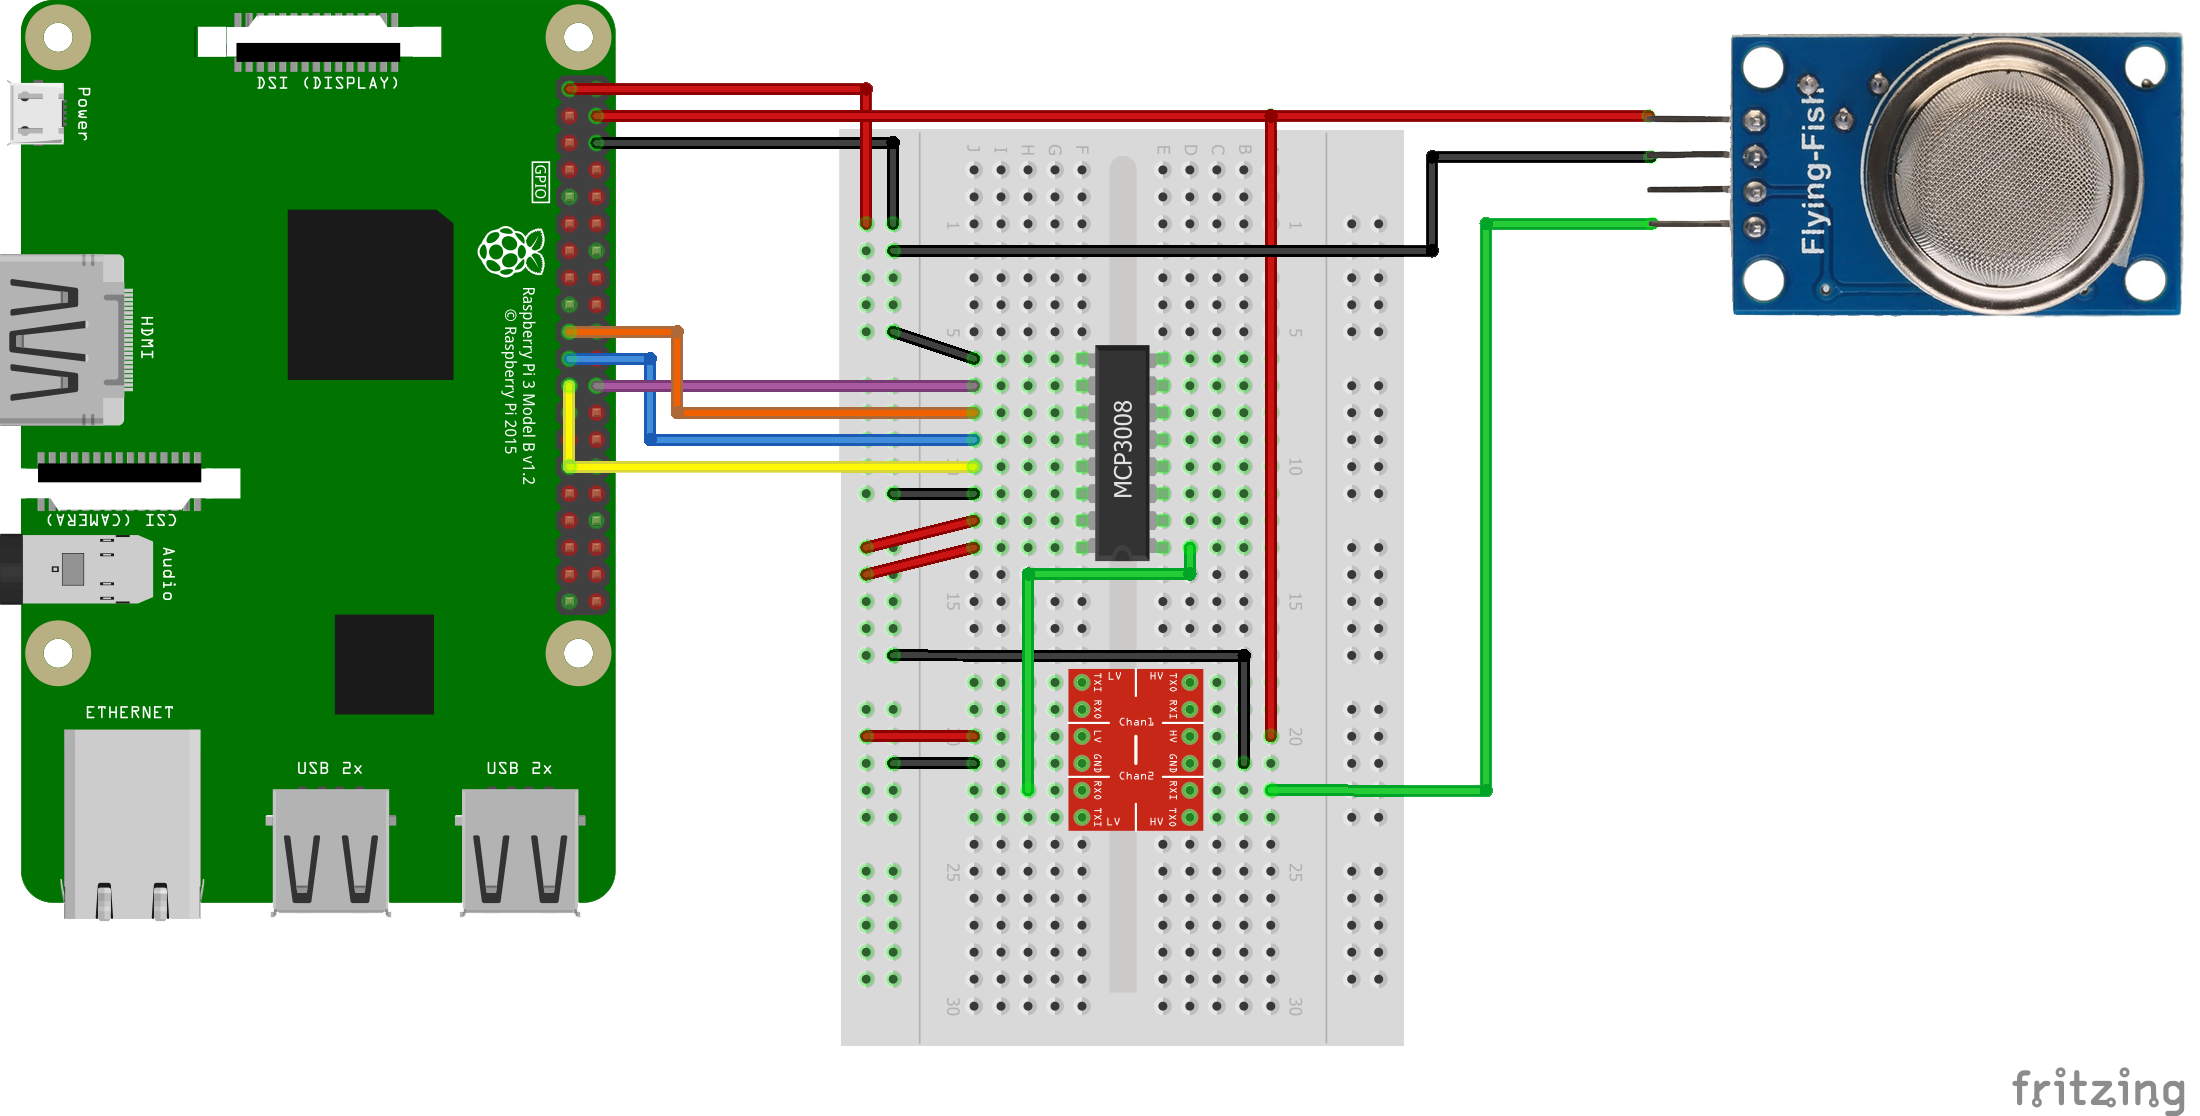
\includegraphics[width=1.00\textwidth]{Raspberry-Pi-Gas-Sensor-MQ2.png}
\caption{Pi wiring}
\label{fig:Pi-MQ2}
\end{figure}

I use the 5V of the Raspberry Pi's. However, an external power supply is recommended if other sensors and modules or input devices (keyboard, mouse, touchscreen) are used. For this, the sensor is simply supplied with current from the external source (HV side of the LLC) and the ground connection (Minus / GND) is connected to GND of the Raspberry Pi.



\subsubsection{Software}

- Python Script

\subsubsection{Soil Moisture}

Tutorials in using a Pi to monistor soil mosture:

\begin{itemize}

\item \href{https://tutorials-raspberrypi.com/measuring-soil-moisture-with-raspberry-pi/}{Simple and Inexpensive Method}

\item \href{moisture-sensor-dfrobothttps://www.switchdoc.com/2018/11/tutorial-capacitive-moisture-sensor-grove/}{Raspberry 3 and Capacitance Sensors -- More Accurate, limited corrosion}

\item \href{https://tutorials-raspberrypi.com/raspberry-pi-capacitive-spoil-moisture-sensor-dfrobot-gravity/}{moisture-sensor-dfrobot?}
\end{itemize}

\subsubsection{Wildlife}

Poacher Cam v7, Chris Kline, panthera.org


\end{document}
